\section{Modello Informativo}

\subsection{Diagramma EER}

l diagramma Entity-Enhanced Relationship descrive la struttura concettuale della base di dati. Le entità sono state individuate a partire dall'analisi dei requisiti funzionali e riflettono lo schema effettivamente implementato su Supabase (PostgreSQL).

\begin{figure}[H]
\centering
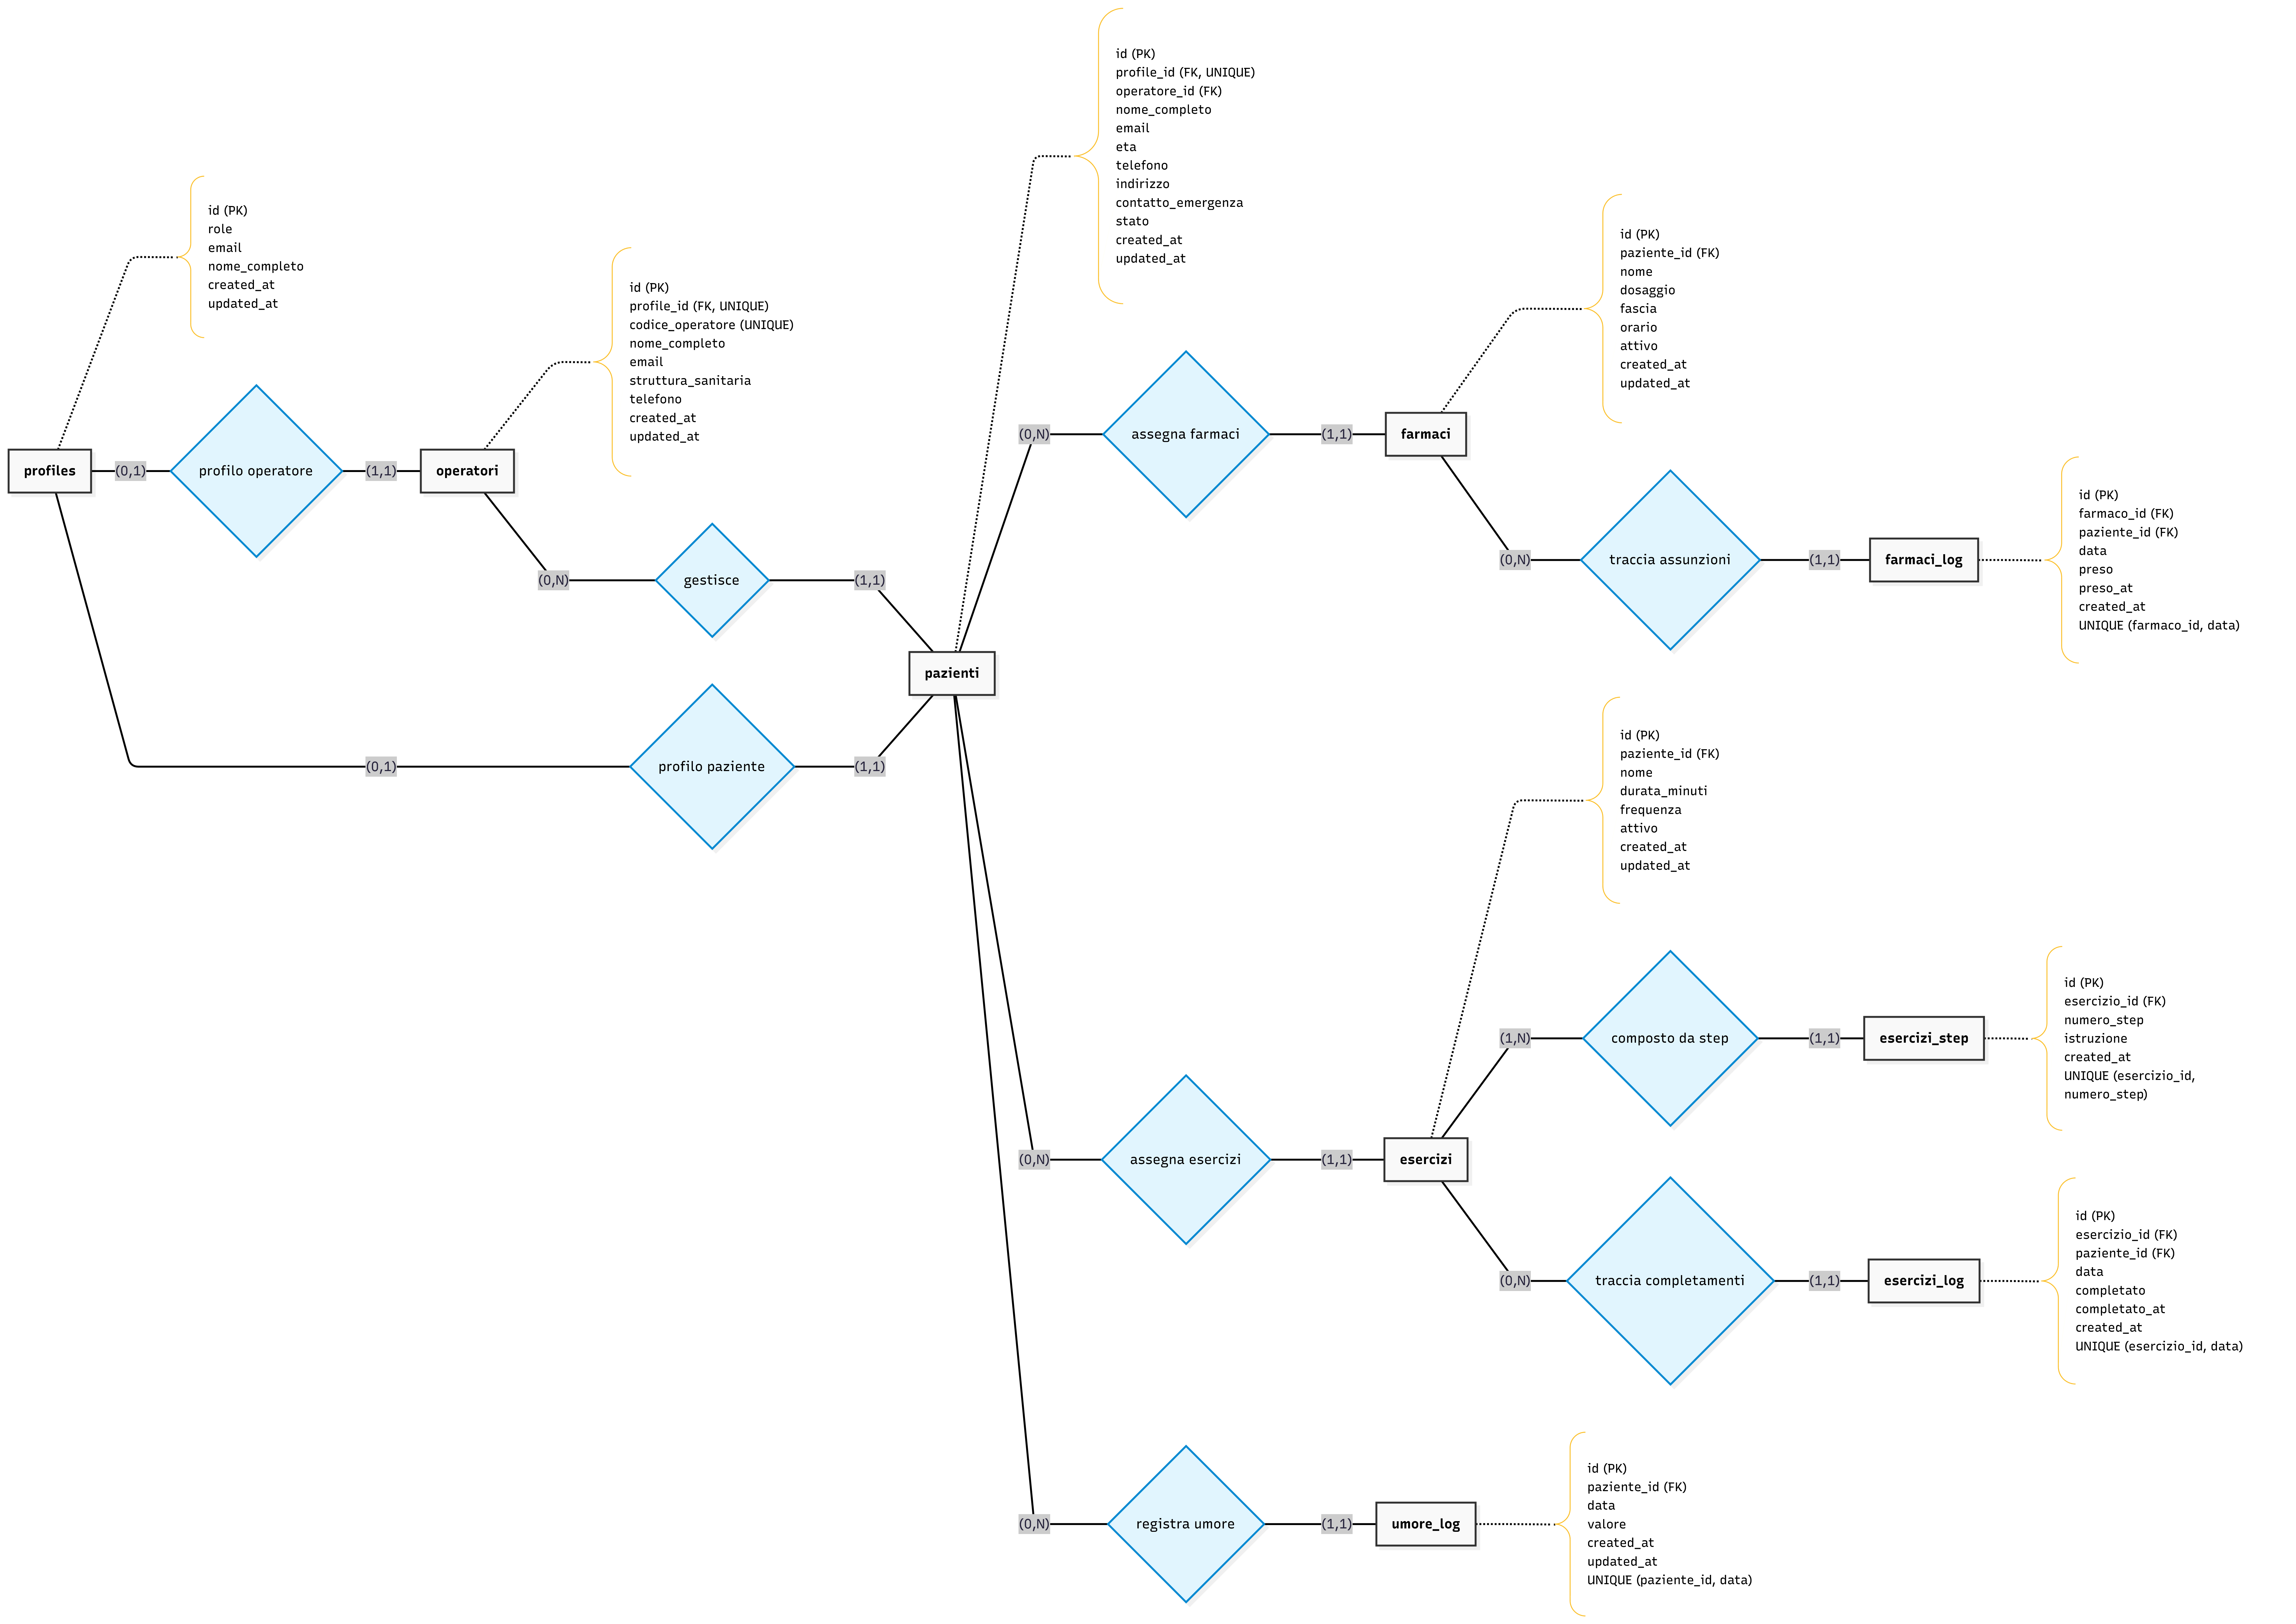
\includegraphics[width=\textwidth,height=0.72\textheight,keepaspectratio]{diagrams/01_eer.png}
\caption{Diagramma EER}
\label{fig:eer}
\end{figure}

\paragraph{Entita' principali}
\begin{itemize}
    \item \textbf{\texttt{profiles}:} profilo applicativo collegato a \texttt{auth.users}. Contiene ruolo, email e nome completo.
    \item \textbf{\texttt{operatori}:} dati dell'operatore sanitario, incluso codice operatore e struttura sanitaria.
    \item \textbf{\texttt{pazienti}:} dati del paziente, operatore assegnato, contatti e stato clinico.
    \item \textbf{\texttt{farmaci}:} farmaci assegnati al paziente, con dosaggio, orario, fascia e stato attivo.
    \item \textbf{\texttt{farmaci\_log}:} registro giornaliero dell'assunzione dei farmaci.
    \item \textbf{\texttt{esercizi}:} esercizi fisici assegnati al paziente.
    \item \textbf{\texttt{esercizi\_step}:} passaggi guidati che compongono un esercizio.
    \item \textbf{\texttt{esercizi\_log}:} registro giornaliero degli esercizi completati.
    \item \textbf{\texttt{umore\_log}:} registrazione giornaliera dell'umore del paziente.
\end{itemize}

\newpage
\subsection{Modello Relazionale}

Il modello relazionale descrive la struttura logica della base di dati, derivato dal diagramma EER. Le tabelle, le chiavi primarie (PK), le chiavi esterne (FK) e i vincoli di integrità referenziale sono rappresentati nel seguente schema:

\begin{figure}[H]
\centering
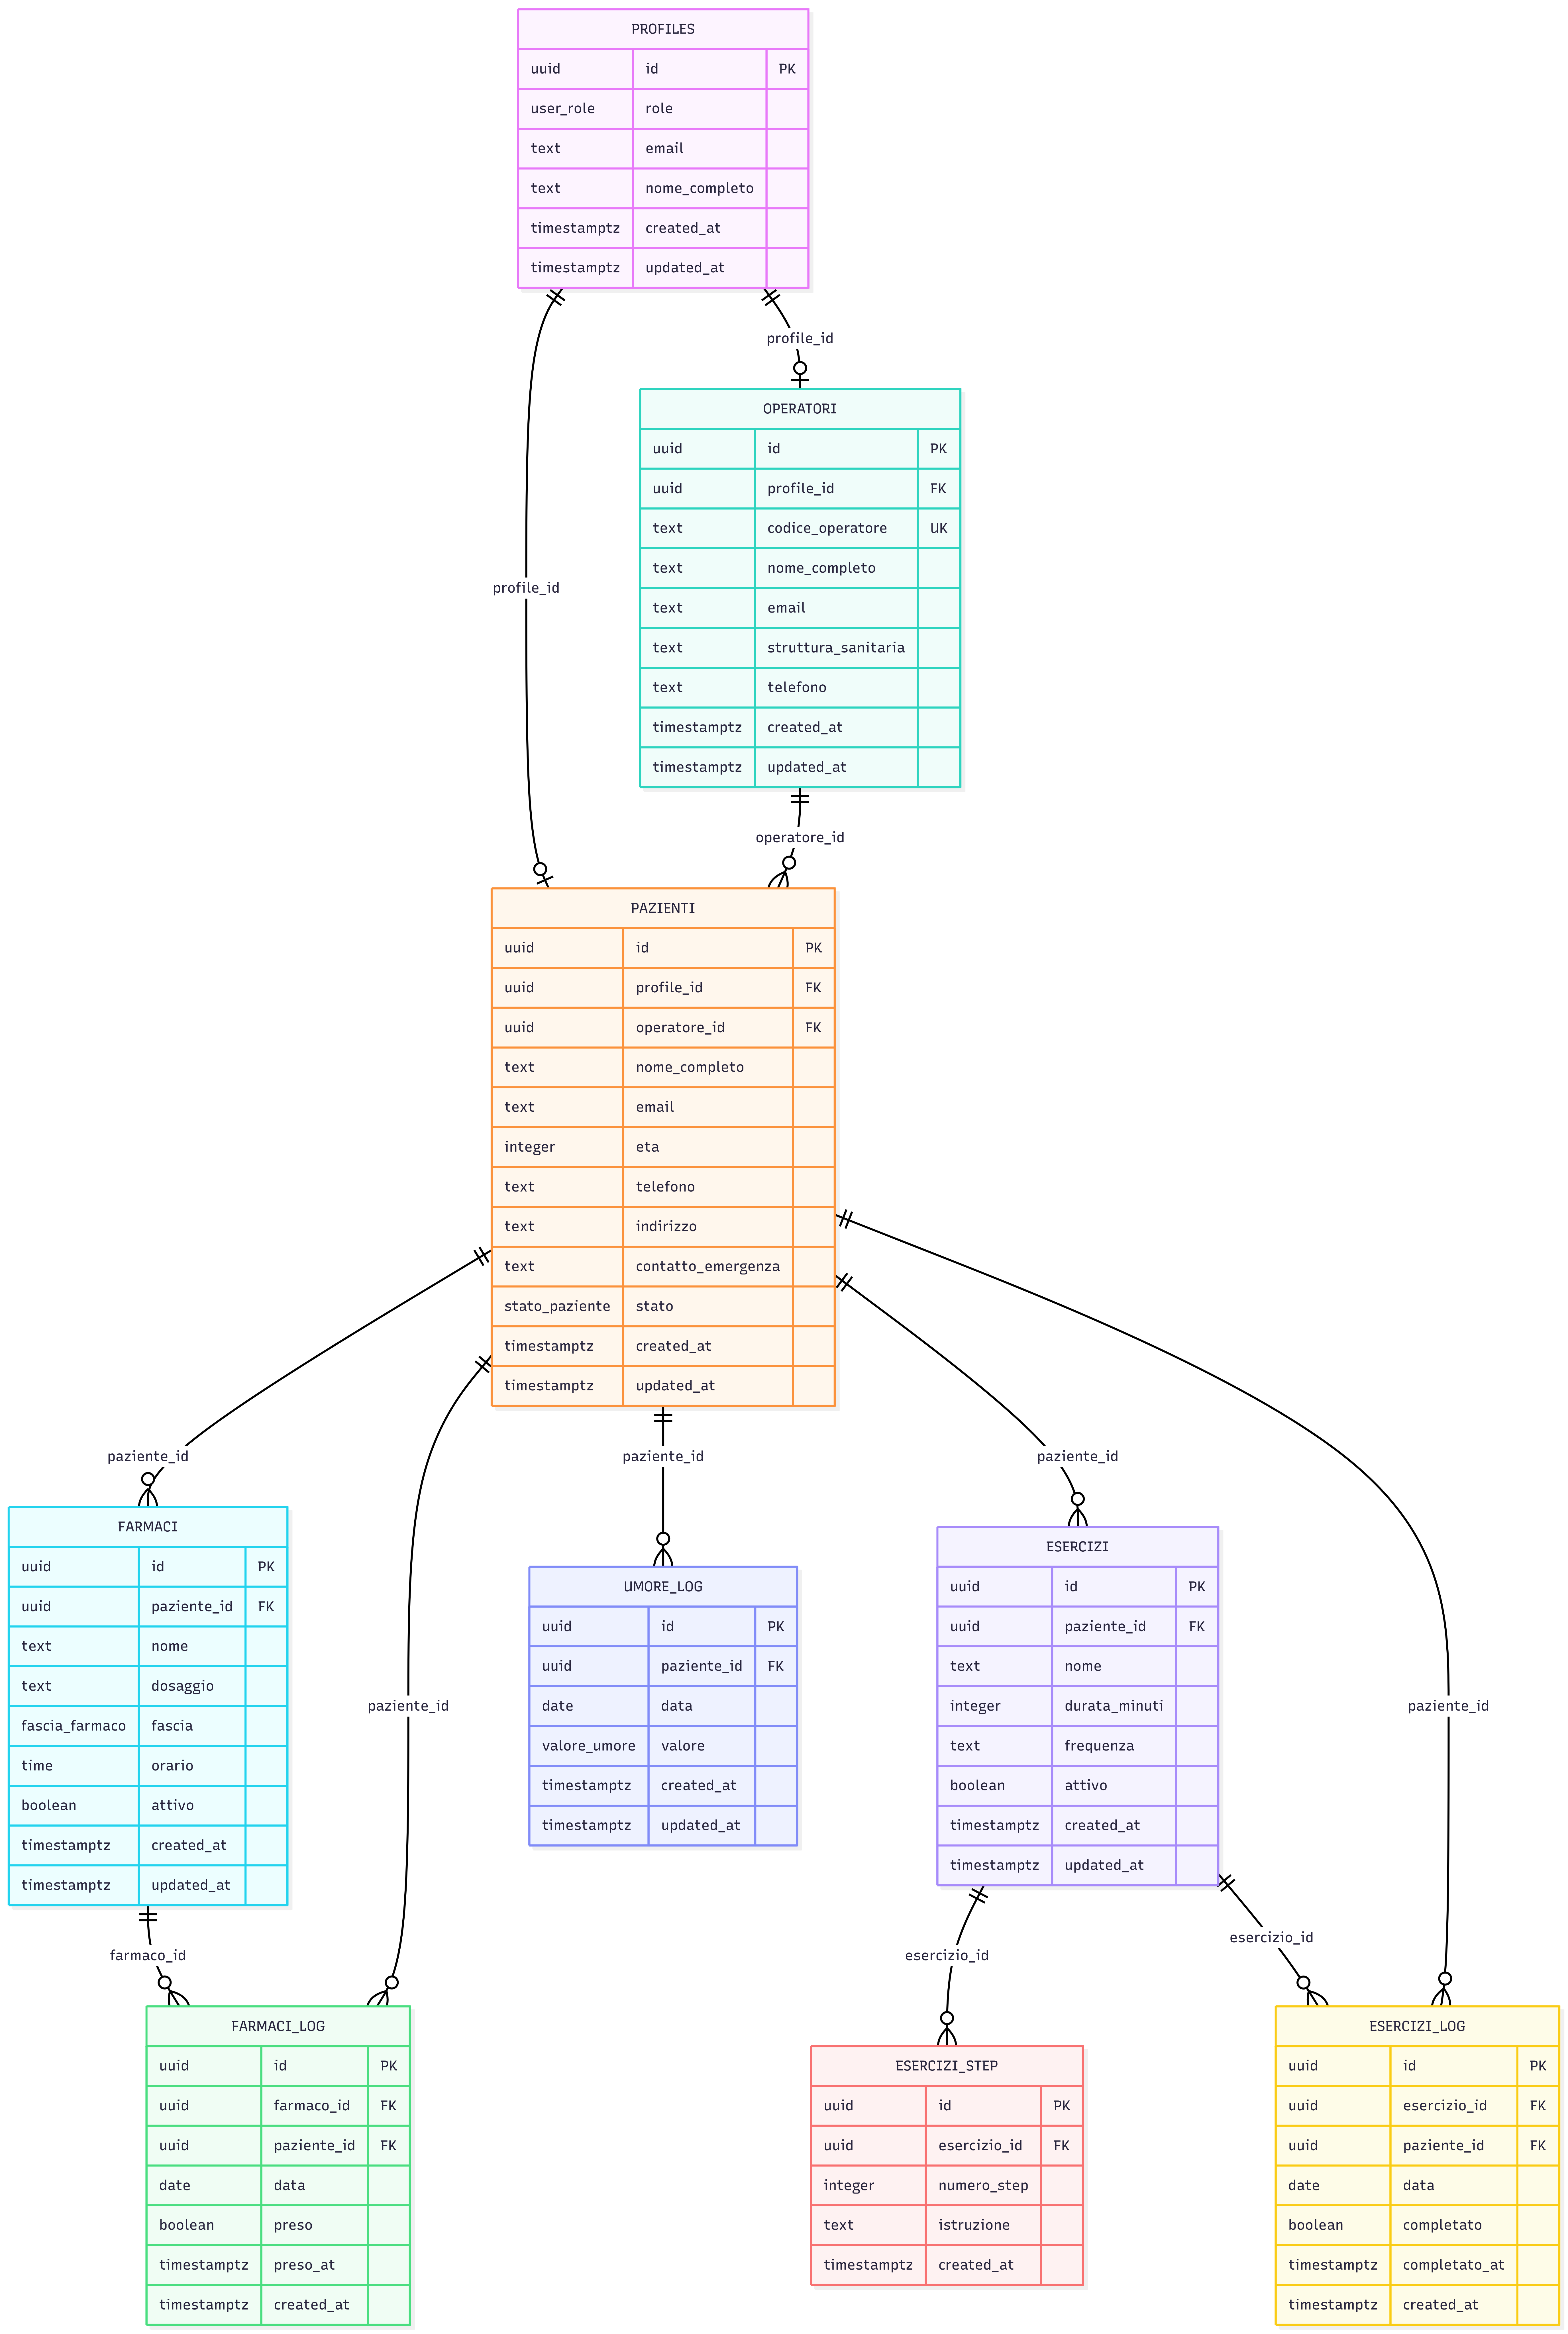
\includegraphics[width=\textwidth,height=0.72\textheight,keepaspectratio]{diagrams/02_modello_relazionale.png}
\caption{Diagramma del modello relazionale con tabelle, PK e FK}
\label{fig:relazionale}
\end{figure}

\subsection{Stima Dimensionale del Database}

\subsubsection{Stima per entita'}
\begin{table}[H]
\centering
\footnotesize
\renewcommand{\arraystretch}{1.25}
\begin{tabular}{|l|r|p{8cm}|}
\hline
\textbf{Tabella} & \textbf{Byte/riga stimati} & \textbf{Note} \\
\hline
profiles & 128 & UUID, ruolo, email, nome e timestamp \\
\hline
operatori & 384 & Dati professionali, codice operatore e contatti \\
\hline
pazienti & 512 & Dati anagrafici, stato e contatto emergenza \\
\hline
farmaci & 208 & Nome, dosaggio, fascia, orario e FK \\
\hline
farmaci\_log & 96 & FK, data, booleano e timestamp \\
\hline
esercizi & 192 & Nome, durata, frequenza e FK \\
\hline
esercizi\_step & 320 & Numero step e istruzione testuale \\
\hline
esercizi\_log & 96 & FK, data, booleano e timestamp \\
\hline
umore\_log & 80 & Data e valore enum testuale \\
\hline
\end{tabular}
\caption{Stima della dimensione media per riga}
\label{tab:stima-byte}
\end{table}

\subsubsection{Tabella di popolamento e crescita}
\begin{table}[H]
\centering
\footnotesize
\renewcommand{\arraystretch}{1.25}
\begin{tabular}{|l|r|r|r|r|}
\hline
\textbf{Tabella} & \textbf{Righe iniziali} & \textbf{Crescita annua} & \textbf{Byte/riga} & \textbf{Dimensione annua stimata} \\
\hline
profiles & 105 & 20 & 128 & $\sim$ 16 KB \\
\hline
operatori & 5 & 1 & 384 & $\sim$ 2 KB \\
\hline
pazienti & 100 & 20 & 512 & $\sim$ 60 KB \\
\hline
farmaci & 500 & 100 & 208 & $\sim$ 122 KB \\
\hline
farmaci\_log & 4.500 & 182.500 & 96 & $\sim$ 17,9 MB \\
\hline
esercizi & 300 & 60 & 192 & $\sim$ 67 KB \\
\hline
esercizi\_step & 900 & 180 & 320 & $\sim$ 337 KB \\
\hline
esercizi\_log & 3.000 & 109.500 & 96 & $\sim$ 10,8 MB \\
\hline
umore\_log & 3.000 & 36.500 & 80 & $\sim$ 3,0 MB \\
\hline
\multicolumn{4}{|r|}{\textbf{Totale dopo un anno}} & $\sim$ \textbf{32,3 MB} \\
\hline
\end{tabular}
\caption{Stima del popolamento e della crescita annua del database}
\label{tab:popolamento}
\end{table}

\subsection{Modello di Visibilita'}

Il modello di visibilità definisce le policy di accesso ai dati in base al ruolo dell'utente autenticato. Il sistema implementa un modello RBAC (Role-Based Access Control) a due livelli: ruolo (operatore vs paziente) e ownership (ogni utente accede solo ai dati di propria competenza).

\begin{figure}[H]
\centering
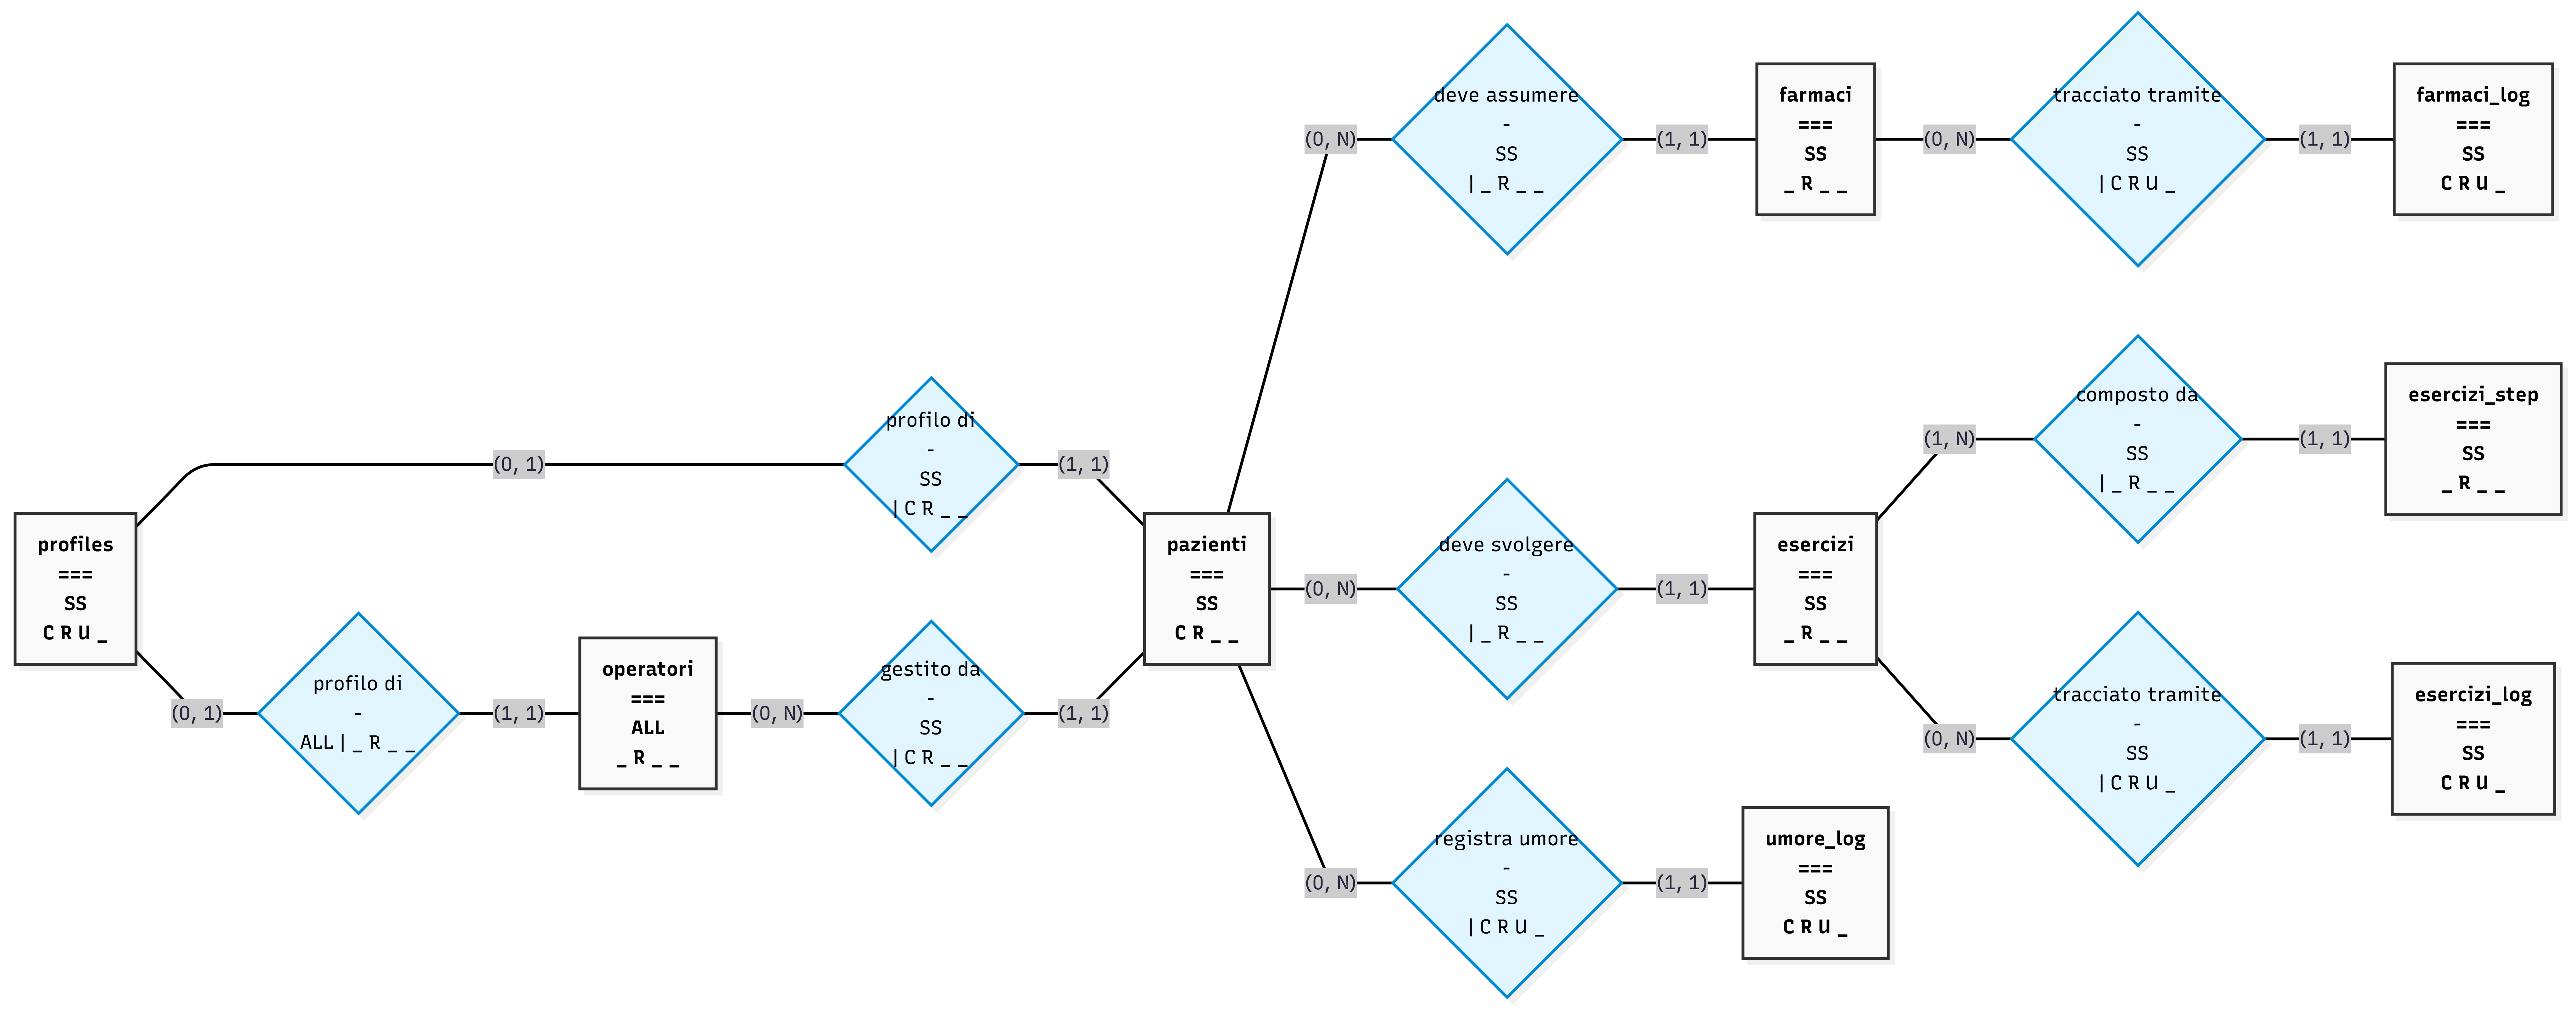
\includegraphics[width=\textwidth,height=0.72\textheight,keepaspectratio]{diagrams/03a_modello_visibilita_paziente.png}
\caption{Modello di visibilita' RLS per il paziente}
\label{fig:visibilita-paziente}
\end{figure}

\begin{figure}[H]
\centering
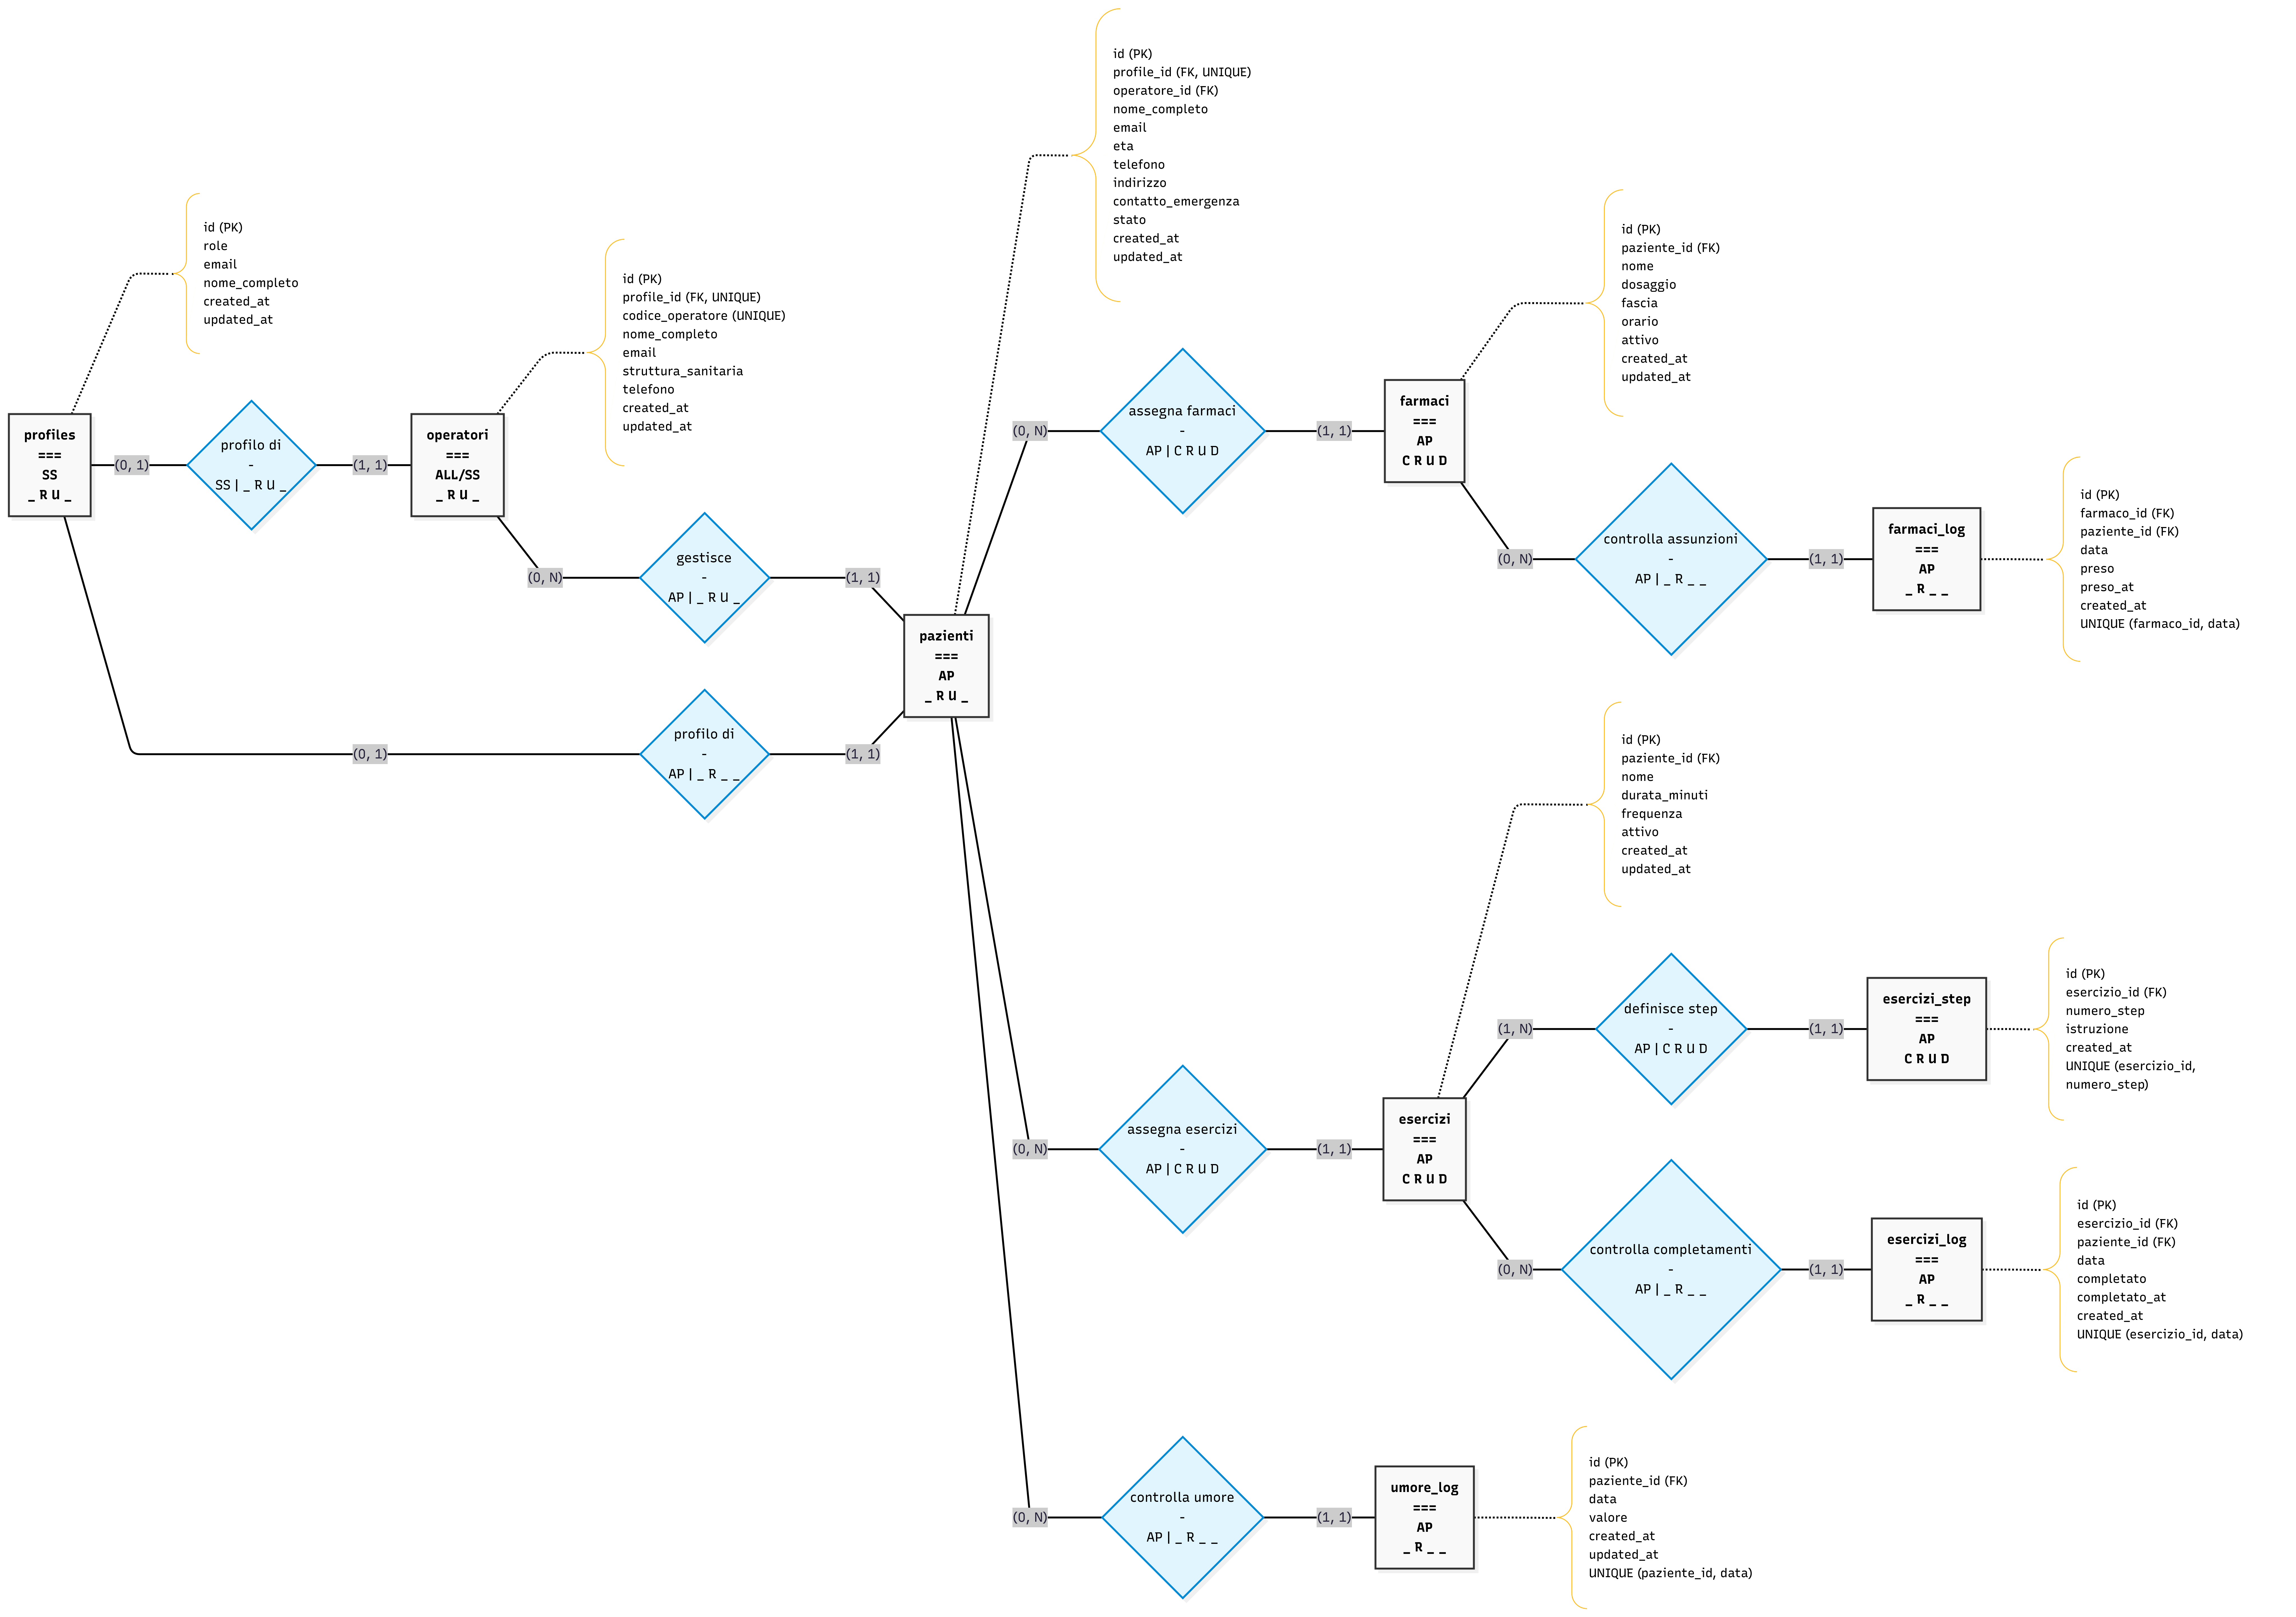
\includegraphics[width=\textwidth,height=0.72\textheight,keepaspectratio]{diagrams/03b_modello_visibilita_operatore.png}
\caption{Modello di visibilita' RLS per l'operatore}
\label{fig:visibilita-operatore}
\end{figure}

\begin{table}[H]
\centering
\footnotesize
\renewcommand{\arraystretch}{1.25}
\begin{tabular}{|p{3.2cm}|c|c|c|c|c|c|c|c|}
\hline
\multirow{2}{*}{\textbf{Risorsa}} & \multicolumn{4}{c|}{\textbf{Operatore}} & \multicolumn{4}{c|}{\textbf{Paziente}} \\
\cline{2-9}
 & C & R & U & D & C & R & U & D \\
\hline
profiles &  & X & X &  &  & X & X &  \\
\hline
operatori &  & X & X &  &  & X &  &  \\
\hline
pazienti &  & X & X &  & X & X &  &  \\
\hline
farmaci & X & X & X & X &  & X &  &  \\
\hline
farmaci\_log &  & X &  &  & X & X & X &  \\
\hline
esercizi & X & X & X & X &  & X &  &  \\
\hline
esercizi\_step & X & X & X & X &  & X &  &  \\
\hline
esercizi\_log &  & X &  &  & X & X & X &  \\
\hline
umore\_log &  & X &  &  & X & X & X &  \\
\hline
\end{tabular}
\caption{Matrice CRUD di visibilita' per ruolo}
\label{tab:visibilita}
\end{table}

\newpage
